\let\negmedspace\undefined
\let\negthickspace\undefined
\documentclass[journal]{IEEEtran}
\usepackage[a4paper, margin=10mm, onecolumn]{geometry}
\usepackage{lmodern} % Ensure lmodern is loaded for pdflatex
\usepackage{tfrupee} % Include tfrupee package

\setlength{\headheight}{1cm} % Set the height of the header box
\setlength{\headsep}{0mm}  % Set the distance between the header box and the top of the text

\usepackage{gvv-book}
\usepackage{gvv}
\usepackage{cite}
\usepackage{amsmath,amssymb,amsfonts,amsthm}
\usepackage{algorithmic}
\usepackage{graphicx}
\usepackage{float}
\usepackage{textcomp}
\usepackage{xcolor}
\usepackage{txfonts}
\usepackage{listings}
\usepackage{enumitem}
\usepackage{mathtools}
\usepackage{gensymb}
\usepackage{comment}
\usepackage[breaklinks=true]{hyperref}
\usepackage{tkz-euclide} 
\usepackage{listings}
% \usepackage{gvv}                                        
\def\inputGnumericTable{}                                 
\usepackage[latin1]{inputenc}                                
\usepackage{color}                                            
\usepackage{array}                                            
\usepackage{longtable}                                       
\usepackage{calc}                                             
\usepackage{multirow}                                         
\usepackage{hhline}                                           
\usepackage{ifthen}                                           
\usepackage{lscape}
\usepackage{tikz}
\usetikzlibrary{patterns}

\begin{document}

\bibliographystyle{IEEEtran}
\vspace{3cm}

\title{3.2.5}
\author{EE25BTECH11064 - Yojit Manral}

\maketitle
% \maketitle
% \newpage
% \bigskip
{\let\newpage\relax\maketitle}
\renewcommand{\thefigure}{\theenumi}
\renewcommand{\thetable}{\theenumi}
\setlength{\intextsep}{10pt} % Space between text and float

\textbf{Question:}\\
Draw a triangle ABC in which BC = 6 cm, CA = 5 cm and AB = 4 cm.\\
\textbf{Solution:}\\
$\rightarrow$ Let
\begin{align}
    a = \norm{\vec{C} - \vec{B}} = 6 cm \\
    b = \norm{\vec{A} - \vec{C}} = 5 cm \\
    c = \norm{\vec{B} - \vec{A}} = 4 cm
\end{align}
$\rightarrow$ By using cosine law in $\triangle$ABC, we get
\begin{align}
    &\cos{B} = \frac{a^{2} + c^{2} - b^{2}}{2ac} \\
    \implies &\cos{B} = \frac{6^2 + 4^2 - 5^2}{2 \times 6 \times 4} \\
    \implies &\cos{B} = \frac{9}{16} \\
    \implies &\angle{B} = \cos^{-1}{\brak{\frac{9}{16}}} \approx 55 \degree
\end{align}
$\rightarrow$ The coordinates of $\triangle$ABC can then be expressed as
\begin{align}
    \vec{A} &= c \myvec{\cos{B}\\\sin{B}} \\
    \vec{B} &= \myvec{0\\0} \\
    \vec{C} &= \myvec{0\\6}
\end{align}
\begin{figure}[h!]
   \centering
   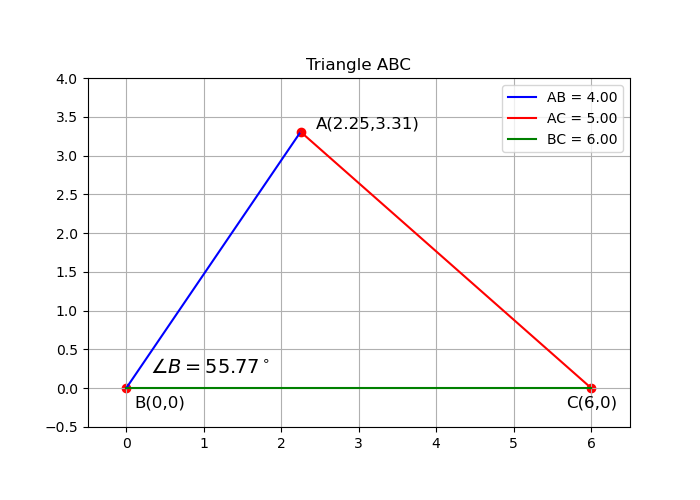
\includegraphics[width=0.8\linewidth]{figs/01.png}
   \caption{Plot of $\triangle$ABC}
   \label{Plot_1}
\end{figure}
\end{document}
